% structure somewhat stolen from http://www.andrew.cmu.edu/user/jonasf/80-413-713/documents/LaTeX_howto.pdf
\documentclass{article}

\usepackage{amssymb,amsmath,amsthm}
\usepackage{tikz}
\usetikzlibrary{positioning,shapes,fit,arrows, backgrounds}



% 													Personal macros and settings
\newcommand {\cat}{%
\mathbf%
}
\newcommand{\ob}[1]{\mathrm{ob}(#1)}
\newcommand {\domain} [ 1 ] {%
\mathrm{dom}(#1)%
}
\newcommand {\codomain } [ 1 ] {%
\mathrm{cod}(#1)%
}
\newcommand {\idarrow} [ 1 ] [ ] {%
\mathbf{1} {#1}%
}

\theoremstyle{definition}
\newtheorem{ch}{Challenge}
\newtheorem{defn}{Definition}[ch]


% 													Document metadata
\title{Solving some problems for Bartosz, chapter 12}
\author{Ludvig Hult}
\date\today


% 													Beg document







% 																CH1 -------------------
\begin{document} 
\maketitle

\begin{ch}
\textit{How would you describe a pushout in the category of C++ classes?}

To attack this this question, first get the terms and keywords right. Let's set down some definitions!

\begin{defn}
Let, $\cat C$, be the category of C++ classes, having
\begin{itemize}
\item $\ob{\cat C}$ be classes in C++
\item Define arrows so that there exists an arrow $f:a\to b$ if $a$ is a subclass of $b$. Otherwise, there is no such arrows from $a$ to $b$.
\end{itemize}
\end{defn}

Some things are clear to see: this is a thin category. It is indeed a category since arrow composition is the same as a inheritence hierarchy. All is good and well. Please remember this, since all diagrams commute in a thin category... Even if I won't use that fact now, thats a good thing to keep in mind! But what is the pushout?

\begin{defn}[pushout]
	A \emph{pushout} is the colimit of a span.
\end{defn}

Which begs for more definitions.What are colimit and spans?

\begin{defn}[span]
	A \emph{span} is category with three objects, and two non-identity arrows: $A \leftarrow B \rightarrow C$.
\end{defn}

Now we are getting somewhere. But what was the colimit nowagain? Well there are so many different definitions of limits and colimits. Personally I use like the definition "a colimit is a limit with all arrows reversed" as a mnenmonic, and the "limit is the terminal object in the cone category" as a philosophical contructs.


I prefer to look at limits and colimits as universal constructions, because that is the easiest to explain. I'll first give it in words and then in a diagram. A colimit of a category $\cat I$ is consctructed by first picking objects and morphism in the category $\cat C$ having the same shape as $I$ (done by a functor $F$, making sure that morphisms compose in the correct way). Then find an object $c$ sucha that there is an injection $i_\alpha$ for all objects $\alpha$ in the image of the functor $F$. The diagram formed by $c, \{i_\alpha\}$ and the image of $F$ must commute. Finally, if therer are any other $c'$ that can be chosen that fulfil the same construction, there is a unique morphism $m$ from $c$ to $c'$ so that the diagram still commute.

This is quite abstract, and also a bit mathematically imprecise, so i'll write you a bicture to convey the mental picture! I'll even use a span for the index category $\cat I$.

\begin{figure}[h]
	\centering
	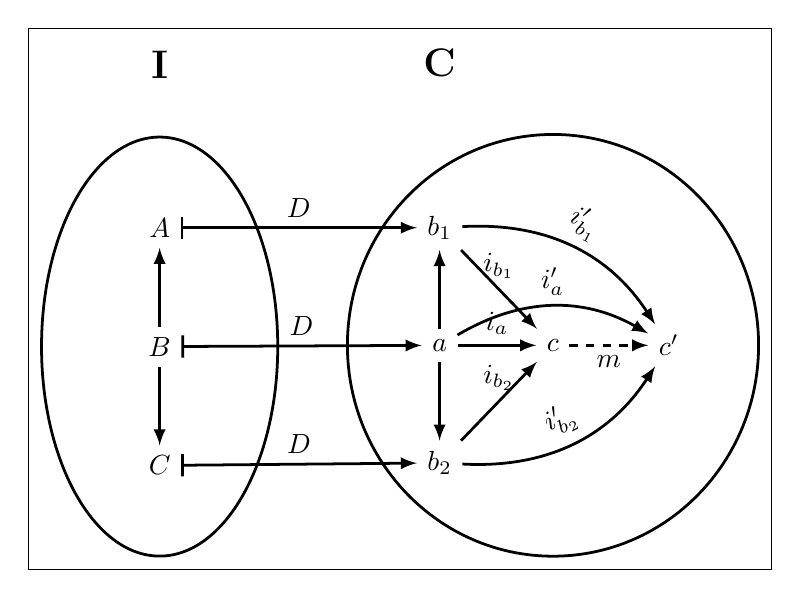
\begin{tikzpicture}[line width=1pt,>=latex, framed]

		% the index category
		\node (ia) {$A$};
		\node[below=of ia] (ib) {$B$};
		\node[below=of ib] (ic) {$C$};
		\node[shape=ellipse,draw=black,minimum size=3cm,fit={(ia) (ic)}] {};
		\node[above=1.5cm of ia,font=\Large] {$\cat I$};
		\draw[->] (ib) -- (ia);
		\draw[->] (ib) -- (ic);
		
		% the C++ category

		%  The image of F
		\node[right=3cm of ia] (cb1) {$b_1$};
		\node[below=of cb1] (ca) {$a$};
		\node[below=of ca] (cb2) {$b_2$};
		\draw[->] (ca) -- (cb1);
		\draw[->] (ca) -- (cb2);
		\draw[|->] (ia) -- (cb1) node[midway,above] {$D$};
		\draw[|->] (ib) -- (ca) node[midway,above] {$D$};
		\draw[|->] (ic) -- (cb2) node[midway,above] {$D$};

		%the co-limiting cone with injections
		\node[right=of ca] (cc) {$c$};
		\draw[->] (cb1) -- (cc) node[midway,above] {$i_{b_1}$};
		\draw[->] (ca) -- (cc) node[midway,above] {$i_{a}$};
		\draw[->] (cb2) -- (cc) node[midway,above] {$i_{b_2}$};

		% another co-cone that is not the co-limit, with injections and factorization
		\node[right=of cc] (ccprime) {$c'$};
		\draw[->] (cb1) to [bend left] node[above, sloped] {$i'_{b_1}$}  (ccprime);
		\draw[->] (ca) to [bend left] node[above, sloped] {$i'_{a}$}  (ccprime);
		\draw[->] (cb2) to [bend right] node[above, sloped] {$i'_{b_2}$} (ccprime) ;

		%the uniquely determined path between co-cone and co-limit
		\draw[->, dashed] (cc) -- (ccprime) node[midway,below] {$m$};


		%the outline of C++ category
		\node[shape=ellipse,draw=black,minimum size=3cm,fit={(cb1) (cb2) (ccprime)}] {};
		\node[above=1.5cm of cb1,font=\Large] {$\cat C$};
	\end{tikzpicture}
	\caption{The pushout in $\cat C$ with defining objects and morphisms.\label{fig:pushout_definition}}
\end{figure}

Now look at figure (\ref{fig:pushout_definition}) and please realize that there are some superflous arrows. Since $\cat C$ is a thin category, it is easy to construct the transitive reduction. Also - in every thin category, every arrows between $c$ and $c'$ must be unique, so it is not important to call $m$ uniquely determined. To emphazise this, I'll stop drawing $m$ as a dashed arrow, and draw it as a solid line instead. And even more: since $\cat C$ is thin, I may also strip the names of all arrows! Finally, since $\cat C$ is thin, all diagrams always commute, and one can freely take the transitive reduction of any diagram without losing information - and this is done in the Figure \ref{fig:pushout_in_c}.


\begin{figure}[h]
	\centering
	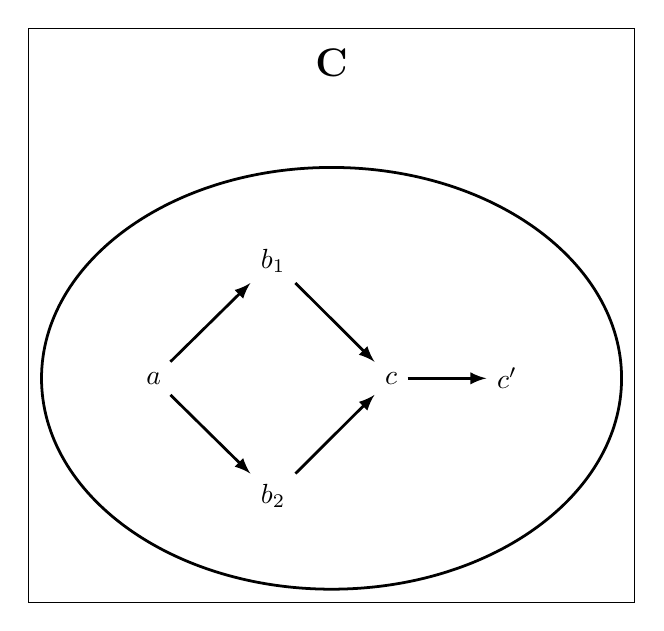
\begin{tikzpicture}[line width=1pt,>=latex, framed]

		%  The image of F
		\node (cb1) {$b_1$};
		\node[below left=of cb1] (ca) {$a$};
		\node[below right=of ca] (cb2) {$b_2$};
		\draw[->] (ca) -- (cb1);
		\draw[->] (ca) -- (cb2);

		%the co-limiting cone with injections
		\node[above right=of cb2] (cc) {$c$};
		\draw[->] (cb1) -- (cc) node[midway,above] {};
		\draw[->] (cb2) -- (cc) node[midway,above] {};

		% another co-cone that is not the co-limit, with injections and factorization
		\node[right=of cc] (ccprime) {$c'$};

		%the uniquely determined path between co-cone and co-limit
		\draw[->] (cc) -- (ccprime) node[midway,below] {};

		%the outline of C++ category
		\node[shape=ellipse,draw=black,minimum size=3cm,fit={(ca) (cb1) (cb2) (ccprime)}] (outline) {};
		\node[above=of outline,font=\Large] {$\cat C$};

	\end{tikzpicture}
	\caption{Transitive reduction of a pushout in $\cat C$.\label{fig:pushout_in_c}}
\end{figure}

Now contemplate the construction of the pushout. Here comes the answer to the challenge: The pushout of $b_1 \leftarrow a \rightarrow b_2$ in $\cat C$ is a C++ class that is the first common superclass of both $b_1$ and $b_2$, and $a$ is inheriting from both $b_1$ and $b_2$. This is the well known situation in programming that can give rise to the diamond problem.
\end{ch}





















% 																CH2 -------------------
\begin{ch}\textit{Show that the limit of the identity functor $Id: C \to C$ is the initial object.}

Okay. Just as before we need to set up seme definitions. Taking the limit of a functor... What even is that? Let's review definitions.

\begin{defn}[Cone over functor $F$]
	 Take a functor $F: \cat I\to \cat C$. Take a constant functor $\Delta_c: \cat I \to \cat C$. If there is a natural transformation $\alpha : \Delta_c \to F$ then the pair $(c,\alpha)$ is a \emph{cone over $F$}.
\end{defn}

\begin{defn}[Limit of a functor $F$]
	 Form a category of cones for $F$ as the following: define the cones as the objects, and we define an arrow $m: (c',\beta) \to (c,\alpha)$ whenever $m$ is uniquely determined by the component wise system of equations $\beta_i = \alpha_i \circ m$. \emph{The limit of $F$ is the terminal object in the cone category}.
\end{defn}

Lets specialize into the case where $F = \mathrm{Id}$! Then $\cat I = \cat C$. If one has an object $c$ in $\cat C$, with unique arrows $p_i: c \to i$ for all other objects $i$ in $\cat C$, then $(c,p)$ is a cone automatically. Here $p: \Delta_c \to \mathrm{Id}_{\cat C}$ is understood as a natural transformation, with components $p_i$. The naturality condition of $p$ is fulfilled trivially. The most important parts of this construction is drawn in Figure \ref{fig:limit_of_id}. 

\begin{figure}[h]
	\centering
	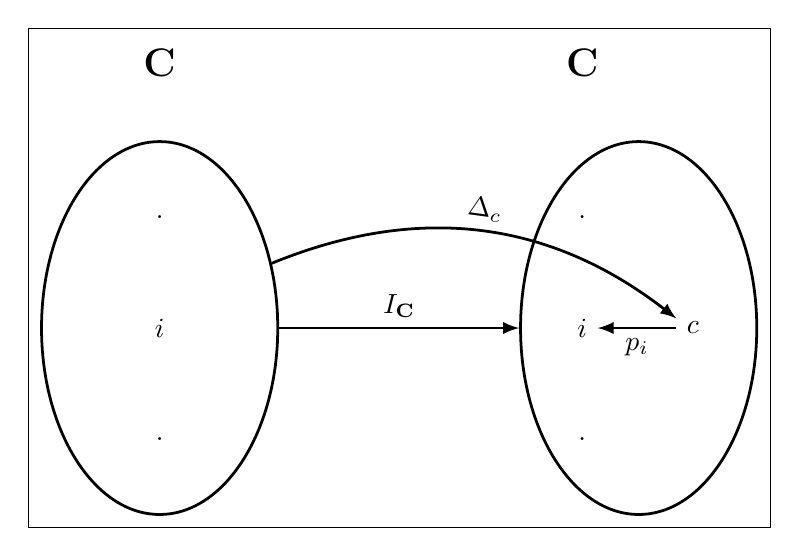
\begin{tikzpicture}[line width=1pt,>=latex, framed]

		% the index category
		\node (ia) {$.$};
		\node[below=of ia] (ib) {$i$};
		\node[below=of ib] (ic) {$.$};
		\node[shape=ellipse,draw=black,minimum size=3cm,fit={(ia) (ic)}] (cleft) {};
		\node[above=1.5cm of ia,font=\Large] {$\cat C$};
		
		%  The image and the cone apex
		\node[right=5cm of ia] (cb1) {$.$};
		\node[below=of cb1] (ca) {$i$};
		\node[below=of ca] (cb2) {$.$};

		%the co-limiting cone with injections
		\node[right=of ca] (cc) {$c$};
		\draw[->] (cc) -- (ca) node[midway,below] {$p_i$};

		%the right C
		\node[shape=ellipse,draw=black,minimum size=3cm,fit={(cb1) (cb2) (cc)}] (cright) {};
		\node[above=1.5cm of cb1,font=\Large] {$\cat C$};

		%´the identity functor
		\draw[->] (cleft) -- (cright)  node[midway,above] {$I_{\cat C}$};
		% the constant functor to the cone apex
		\draw[->] (cleft) to [bend left] node[above, sloped] {$\Delta_{c}$} (cc) ;

	\end{tikzpicture}
	\caption{Important parts of the limit definiton. To the left, we have an index category. To the right, there is a category in which we take the limit. They are connected via a diagram functor, wich in this case is the identity functor $I_{\cat C}$. The object $c$ is a cone apex, which is connected to the image of the diagram functor via projections $p_i$. \label{fig:limit_of_id}}
\end{figure}

Now consider the initial object $0$ of $\cat C$. Following from the definiton of the initial object, there is such unique arrows $p_i: 0 \to i$. By the previous paragraph, $(0,p)$ is a cone. Also, there must be a unique arrow $m: 0 \to c'$ for any other cone $(c',p')$, also by the definition of terminal objects. Since $m$ and $p_{c'}$ are unique, they must also automatically satisfy $p_i = p'_i \circ m$. So there is a unique arrow $m: (0,p) \to (c',p')$ in the category of cones over $\mathrm{Id}$. 

Thus, we arrive at the conclusion that $0$ is the limit we are seeking. This completes the challenge.
\end{ch}






















%																CH3 --------------------------------
\begin{ch}\textit{Subsets of a given set form a category. A morphism in that category is defined to be an arrow connecting two sets if the first is the subset of the second. What is a pullback of two sets in such a category? What’s a pushout? What are the initial and terminal objects?}\end{ch}

I'll reason quite fast here, since there is not too much complicated details... Call the category $\cat C$.

First take the pullback. It is shown in Figure \ref{fig:pullback_in_PS}. From the diagram, we see that the pullback $d \subseteq a$, $d \subseteq b$, $d \subseteq c$. But also that for all other $d'$  that are subsets to$a$, $b$ and $c$, $d' \subseteq d$. Or in other words, $d$ is the largest set that contains all the elements common to both $a$, $b$ and $c$. That is - $d = a \cup b \cup c$. But this holds too much information! Since $a \subseteq b$ and $c \subseteq b$, it suffice to define characterize $d = a \cup b$.

\begin{figure}[h]
	\centering
	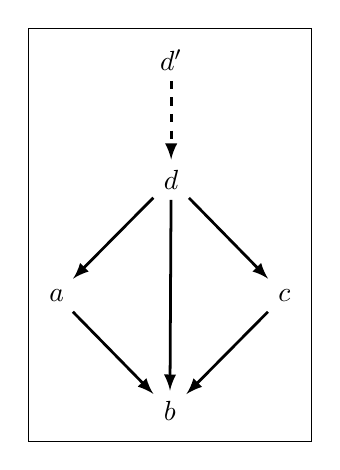
\begin{tikzpicture}[line width=1pt,>=latex, framed]

		\node (d) {$d$};
		\node[below left=of d] (a) {$a$};
		\node[below right=of d] (c) {$c$};
		\node[below right=of a] (b) {$b$};
		\node[above=of d] (dprime) {$d'$};

		\draw[->] (d) -- (a);
		\draw[->] (d) -- (b);
		\draw[->] (d) -- (c);
		\draw[->,dashed] (dprime) -- (d);

		\draw[->] (a) -- (b);
		\draw[->] (c) -- (b);
	\end{tikzpicture}
	\caption{The limit of the diagram $a \rightarrow b \leftarrow c$. $d$ is the \emph{pullback} if it is chosen so that so that all other cone apexes chosen so that there is unique factorizations in a proper sense. \label{fig:pullback_in_PS}}
\end{figure}

For the pushout, the reasoning is very much similar. The diagram looks like Figure \ref{fig:pushout_in_PS}. The pushout $c = 1 \cap 2$.

\begin{figure}[h]
	\centering
	\begin{tikzpicture}[line width=1pt,>=latex, framed]

		\node (d) {$c$};
		\node[below left=of d] (1) {$a$};
		\node[below right=of d] (2) {$c$};
		\node[below right=of a] (3) {$b$};
		\node[above=of d] (dprime) {$c'$};

		\draw[<-] (d) -- (a);
		\draw[<-] (d) -- (b);
		\draw[<-] (d) -- (c);
		\draw[<-,dashed] (dprime) -- (d);

		\draw[<-] (a) -- (b);
		\draw[<-] (c) -- (b);
	\end{tikzpicture}
	\caption{The limit of the diagram $1 \leftarrow 2 \rightarrow 3$. $c$ is the \emph{pushout} if it is chosen so that so that all other cone apexes chosen so that there is unique factorizations in a proper sense. \label{fig:pushout_in_PS}}
\end{figure}

The initial object $0$ needs to have a unique arrow to every other object in the category. Since the category is thin, it is trivially unique. What object has an arrow to any other object? It means $0 \subseteq a \forall a \in \cat C$. The only such set is the empty set. So $0 = \emptyset$.

The terminal object must dually be the superset of all other sets in the category. Only the whole original set fulfils this.






















% 																CH4 -------------------
\begin{ch}\textit{Can you guess what a coequalizer is?}\end{ch}

This is actually a quite funny question. Can I guess? Would "no" do for an answer? So I guess the correct answer must be "yes". A coequalizer must be the dual notion of a equalizer. Remember that an equalizer is the limit of the diagram $D$ from an index category $I$ with two objects $a$ and $b$ and two arrows $f$ and $g$ from $a$ to $b$, $a\rightrightarrows_f^g b$. 

The dual notion is given by the co-limit of the opposite diagram. Lets first formulate it, and then see what it actually means. 

\begin{defn}[Coequalizer]
A \emph{coequalizer} is the co-limit of the diagram $D$ from an index category $\cat I^{op}$, where $\cat I$ is represented by $a\rightrightarrows_f^g b$.
\end{defn}

We worked through the co-limit definition in the text above - so lets just draw the relevant diagram with central objects and arrows drawn. The whole picture in its glory is what I call Figure \ref{fig:coequalizer}. You read the picture like this: given $a$,$b$,$f$,$g$, you call $c$ a coequalizer if there are arrows (called injections) $p$ and $q$, and so that all other $c'$ with corresponding injections $p'$ and $q'$ factorize over some  $m$ determined uniquely by the injections $p'$ and $q'$.

\begin{figure}[h]
	\centering
	\begin{tikzpicture}[line width=1pt,>=latex, framed]

		\node (c) {$c$};
		\node[below left=of c] (a) {$a$};
		\node[below right=of c] (b) {$b$};

		\draw[->] (b) to [bend left] node[below, sloped] {$f$} (a) ;
		\draw[->] (b) to node[above, sloped] {$g$} (a) ;

		% injections
		\draw[<-] (c)-- node[above] {$p$} (a) ;
		\draw[<-] (c) -- node[above] {$q$} (b);

		% an other co-cone
		\node[above=of d] (cprime) {$c'$};
		\draw[->] (a) to [bend left] node[above, sloped] {$p'$} (cprime) ;
		\draw[->] (b) to [bend right] node[above, sloped] {$q'$} (cprime) ;
		\draw[->,dashed] (c) -- node[right] {$m$} (cprime);

	\end{tikzpicture}
	\caption{This diagram defines $c$ to be coequalizer for $a$,$b$,$f$,$g$, given that all arrows commutes, and that $m$ is uniquely determined by all the other arrows..\label{fig:coequalizer}}
\end{figure}

First, you must realize that the whole construction is overdetermined. The arrows $q$ and $q'$ are automatically detemined by $p$ and $p'$. They may be omitted with no loss of information.

Next, realize that the construction gives the equation $p \circ g = p \circ f$.

Thirdly, realize thatfor every $p'$ we must have  $p' = m \circ p$, where $m$ is uniquely determined by $p'$. This can be interpreted as $p$ in a sense is a arrow that does not lose any relevant information about $a$.

Exactly what this equation really gives is of course determined by what category that the coqualizer is defined in. My own ability and curiosity doesn't take me any longer here.




















% 																CH5 -------------------
\begin{ch}\textit{Show that, in a category with a terminal object, a pullback towards the terminal object is a product.}

Start off by remembering the definitions. The "pullback towards the terminal object" is the limit of a diagram from a cospan category - a category of the shape $o_1 \leftarrow o_2 \rightarrow o_3$. A product is the limit of the diagram from a discrete category with two objects - two objects and no arrows except the identity arrows.

So lets start with the product, and then show that nothing changes when we introduce the necessary parts to change that construction into a pullback towards the terminal object. The product construction is in Figure \ref{fig:product_in_c}. I let the image of the diagram be two objects $a$ and $b$. I'll call the product $a\times b$. Projections from the product to $a$ and $b$ will be called $\mathrm{fst}$ and $\mathrm{snd}$. An other cone over the diagram will be called $d$, and its projections will be called $f$ and $g$. The factorizer determined by $f$ and $g$ will be called $<f,g>$.

\begin{figure}[h]
	\centering
	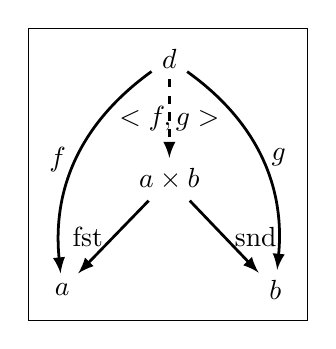
\begin{tikzpicture}[line width=1pt,>=latex, framed]

		%the image of the diagram
		\node[] (a) {$a$};
		\node[right=of a] (one) {};
		\node[right=of one] (b) {$b$};



		%the limiting cone
		\node[above=of one] (ab) {$a\times b$};
		\draw[->] (ab) --  node[left] {$\mathrm{fst}$} (a);
		\draw[->] (ab) -- node[right] {$\mathrm{snd}$} (b) ;

		% another cone, and the unique factorizer
		\node[above=of ab] (d) {$d$};
		\draw[->,dashed] (d) -- node[] {$<f,g>$} (ab);
		\draw[->] (d) to [bend right] node[left] {$f$} (a) ;
		\draw[->] (d) to[bend left] node[right] {$g$} (b) ;


	\end{tikzpicture}
	\caption{A product. The line for $<f,g>$ is dashed to indicate that is uniquely determined. \label{fig:product_in_c}}
\end{figure}

Next, I'll add objects and arrows into the construction, to show that all the newly introduced arrows are suprflous - they do not introduce any new information into the picture! Figure \ref{fig:pullback_in_c} shows this!

\begin{figure}[h]
	\centering
	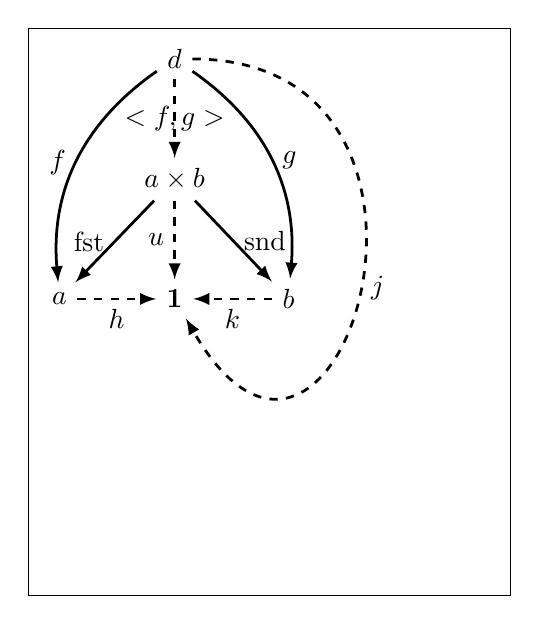
\begin{tikzpicture}[line width=1pt,>=latex, framed]

		%the image of the diagram
		\node[] (a) {$a$};
		\node[right=of a] (one) {$\idarrow$};
		\node[right=of one] (b) {$b$};
		\draw[->,dashed] (a) -- node[below] {$h$} (one);
		\draw[->,dashed] (b) -- node[below] {$k$} (one);


		%the limiting cone
		\node[above=of one] (ab) {$a\times b$};
		\draw[->] (ab) --  node[left] {$\mathrm{fst}$} (a);
		\draw[->,dashed] (ab) --  node[left] {$u$} (one);
		\draw[->] (ab) -- node[right] {$\mathrm{snd}$} (b) ;

		% another cone, and the unique factorizer
		\node[above=of ab] (d) {$d$};
		\draw[->,dashed] (d) -- node[] {$<f,g>$} (ab);
		\draw[->] (d) to [bend right] node[left] {$f$} (a) ;
		\draw[->] (d) to[bend left] node[right] {$g$} (b) ;
		\draw[->, dashed] (d) to [out=0,in=300,looseness=3] node[right] {$j$} (one);

	\end{tikzpicture}
	\caption{A pullback towards the terminal object. The arrows $u$, $h$, $k$, $j$ us uniquely determined, by the definition of a limiting object $\idarrow$. \label{fig:pulback_in_c}}
\end{figure}

This final thing to clarify before we are done is to say that the figiures \ref{fig:product_in_c} and \ref{fig:pullback_in_c} are identical. First the image of a diagram from a copsan means that I need to introduce a new object (in this exercise that object is $\idarrow$) and arrows to that object (which I will call $h$ and $k$). In general, one can choose and $h$ and $k$, but since the codomain of those arrows are $\idarrow$, they are actually uniquely determined. No new information introduced into the construction here! Next both cones (the limiting product cone and the other cone $d$) need a new projection into the new object $\idarrow$. They are uniquely determined too - so there is no new information here either. Finally, we demand commutation in the whole picture, and that is automatically satisfied following from unicity of all the newly introduced arrows!

Thus - we are finised!
\end{ch}


















% 																CH6 -------------------
\begin{ch}\textit{Similarly, show that a pushout from an initial object (if one exists) is the coproduct.} 

This proof is so identical to the one above that I won't bother to do it with images and all.

Start with a coproduct $a \sqcup b$ with cofactors $a$ and $b$. There must be unique arrows to $a$, $b$ and $a \sqcup b$ from the initial object $\mathbf 0$. That means that $a \sqcup b$ is also a co-cone of the pushout from $mathbf 0$ to $a$ and $b$. It is also the universal co-cone, since it was that deisregarding the unique arrows that we introduced. 

I think this reasoning is sufficient to understand the situation.

The end.\end{ch}

\end{document}
